\section{Passo 3 — Criar a rodada e enviar as exportações}
\label{sec:passo3}

\subsection*{Objetivo}
Registrar uma coleta datada e carregar nela os arquivos exportados de cada base.

\begin{figure}[H]
\centering
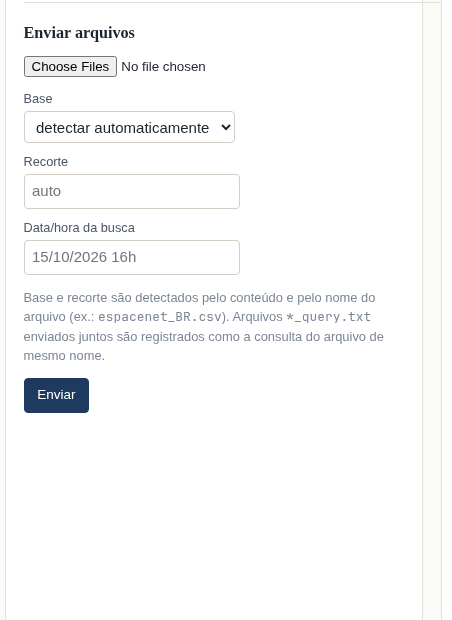
\includegraphics[width=0.62\linewidth]{img/03_upload_painel.png}
\caption{Formulário de envio de arquivos, na própria tela da rodada. O nome do arquivo define a
base e o recorte; a data de execução registra quando a busca foi feita.}
\label{fig:upload}
\end{figure}

\subsection*{O que fazer}
\begin{enumerate}
\item No estudo, clique em \textbf{Nova rodada} e informe um rótulo (por exemplo, a data da coleta).
\item Envie os arquivos de uma vez. O nome deve seguir o padrão \campo{<base>\_<recorte>.csv} ou
      \campo{.txt}: \campo{lens\_nucleo.csv}, \campo{espacenet\_nucleo.csv},
      \campo{google\_nucleo.csv}, \campo{darwent\_nucleo.txt}.
\item Se a exportação não trouxer a consulta no cabeçalho, envie também
      \campo{lens\_query.txt} com o texto da consulta.
\item Informe a data/hora de execução e confirme o envio.
\end{enumerate}

\subsection*{Como interpretar}
Cada arquivo se torna um registro com três informações: \textbf{base} (lens, espacenet, google,
darwent, inpi), \textbf{recorte} (o conjunto; \campo{nucleo} é o principal) e \textbf{número de
registros lidos}. A aplicação ignora arquivos de ``concepts'' e arquivos fora do padrão --- se um
arquivo não aparecer na lista, o problema é o nome.

O recorte não é decoração: a consolidação usa apenas o recorte definido em \campo{core\_recorte}. Um
arquivo nomeado com outro recorte entra no estudo, mas fica fora da base unificada.

\begin{nota}[Proveniência]
Guardar a consulta permite responder ``de onde veio este número?'' meses depois. A tela de rodada
marca com aviso as exportações sem consulta declarada; isso não impede o cálculo, mas impede a
reprodutibilidade.
\end{nota}

\begin{alerta}[Erro comum]
Reenviar arquivos na mesma rodada sem marcar \textbf{substituir}. Os documentos são somados e o
PRISMA passa a contar duplicatas que não são famílias.
\end{alerta}

\subsection*{Checkpoint}
\marcador\; A rodada lista quatro arquivos e o total de registros lidos é \num{15}.
